\documentclass{beamer}

\newcommand{\cmd}[1]{\textbf{\texttt{#1}}}
\newcommand{\pkg}[1]{\texttt{#1}}
\newcommand{\env}[1]{\texttt{#1}}
\newcommand{\opt}[1]{\textsl{#1}}

\usepackage{beamerthemesplit}
\beamertemplatenavigationsymbolsempty
\setbeamertemplate{footline}[frame number]{}

\usepackage{graphicx}
\usepackage{color}
\usepackage{listings}
\usepackage{verbatim}
\usepackage{setspace}
\usepackage{url}
\usepackage{hyperref}

\usepackage{fontspec}
\setmonofont{Latin Modern Mono}
\setsansfont{TeX Gyre Heros}

\lstset{breakatwhitespace=true,
language=C++,
basicstyle=\footnotesize\ttfamily,
keywordstyle=\color{blue}\ttfamily,
stringstyle=\color{red}\ttfamily,
commentstyle=\color{brown}\ttfamily,
morecomment=[l][\color{magenta}]{\#}keepspaces=true,
breaklines=true,
tabsize=3,
showstringspaces=false,
extendedchars=true,
frame=single,
escapeinside=§§
}

\newcommand*{\vcenteredhbox}[1]{\begingroup
\setbox0=\hbox{#1}\parbox{\wd0}{\box0}\endgroup}

\usepackage{tikz}
\usetikzlibrary{matrix}
\usepackage{ragged2e}

\tikzstyle{component} = [rectangle, rounded corners, minimum width=5cm, text width=4cm, minimum height=0.8cm,text centered, draw=black, fill=red!30]
\tikzstyle{repo} = [rectangle, minimum width=5cm, text width=4cm, minimum height=0.8cm, text centered, draw=black, fill=orange!30]
\tikzstyle{newrepo} = [rectangle, minimum width=5cm, text width=4cm, minimum height=0.8cm, text centered, draw=black, fill=orange!60]

\tikzstyle{arrow} = [thick,->,>=stealth]
\tikzstyle{darrow} = [thick,<->,>=stealth]

\newcommand*{\abox}[1]{\framebox{\hbox to 0.5cm{\texttt\{{\\hss#1\hss}}}}

\title{OME Files C++ status}
\author{Roger Leigh}
\date{May 2017}

\begin{document}

\begin{frame}[plain,fragile]
  \centering
  
\includegraphics[width=0.6\textwidth]{figures/ome-files}
  \titlepage

  \begin{center}
    \textsl{Progress over the last year and upcoming features}
  \end{center}
\end{frame}

\begin{frame}[plain,fragile]
  \frametitle{Introduction}
  \begin{center}
    
\includegraphics[width=0.6\textwidth]{figures/ome-files}
  \end{center}
  \bigskip

  What \emph{is} OME Files?
  \bigskip

  OME Files is a reference implementation of the OME Metadata Model
  and the OME-TIFF file format.

  \begin{itemize}
  \item Broad API compatibility with Bio-Formats Java
  \item Read and write support for OME-TIFF and TIFF
  \item OME Files: reader and writer API
  \item OME Model: model and metadata API
  \end{itemize}
  
\end{frame}

\begin{frame}[fragile]
  \frametitle{Component splitting: completed}
  \begin{center}
    \begin{tikzpicture}[y=-1cm]
      \onslide<1->{
        \node (bfrepo) [repo] {bioformats.git};
        \node (c1) [component, below of=bfrepo, yshift=-0.3cm] {ome-compat};
        \node (c2) [component, below of=c1, yshift=-0.3cm] {ome-common};
        \node (c3) [component, below of=c2, yshift=-0.3cm] {ome-xml};
        \node (c4) [component, below of=c3, yshift=-0.3cm] {ome-bioformats};
        \node (c5) [component, below of=c4, yshift=-0.3cm] {ome-qtwidgets};

        \draw [thick] (bfrepo.south) -- (c1.north);
        \draw [thick] (c1.south) -- (c2.north);
        \draw [thick] (c2.south) -- (c3.north);
        \draw [thick] (c3.south) -- (c4.north);
        \draw [thick] (c4.south) -- (c5.north);
      }
      \onslide<2->{
        \node (sb) [repo, right of=bfrepo, xshift=5cm] {ome-cmake-superbuild.git};
        \node (commonrepo) [repo, right of=c2, xshift=5cm, yshift=0.7cm] {ome-common-cpp.git};
        \node (xmlrepo) [newrepo, right of=c3, xshift=5cm] {ome-model.git};
        \node (filesrepo) [repo, right of=c4, xshift=5cm] {ome-files-cpp.git};
        \node (qtrepo) [repo, right of=c5, xshift=5cm] {ome-qtwidgets.git};

        \draw [arrow] (bfrepo) -- (sb);
        \draw [arrow] (c1) -- (commonrepo);
        \draw [arrow] (c2) -- (commonrepo);
        \draw [arrow] (c3) -- (xmlrepo);
        \draw [arrow] (c4) -- (filesrepo);
        \draw [arrow] (c5) -- (qtrepo);
      }
    \end{tikzpicture}
  \end{center}
\end{frame}

\begin{frame}[fragile]
  \frametitle{Performance testing}

  \begin{itemize}
  \item Profiling of C++, Java and JNI (JACE)
  \item Real-world data-sets:
    \begin{itemize}
    \item Simple 5D volume (small, limited metadata)
    \item Plate (many images, large pixeldata size)
    \item ROI (many ROIs, large metadata size)
    \end{itemize}
  \item Detailed investigation with call and cache profiling (\texttt{valgrind}
    with \texttt{callgrind} and \texttt{cachegrind})
  \item Ongoing work: tiling performance
  \end{itemize}
  
  Repository: \url{https://github.com/openmicroscopy/ome-files-performance/tree/0_1}\\
  Preprint: \url{http://biorxiv.org/content/early/2017/03/09/088740}\\
  Zenodo: \url{https://zenodo.org/record/559270}
\end{frame}

\begin{frame}[fragile]
  \frametitle{Performance testing results}
  \begin{centering}
    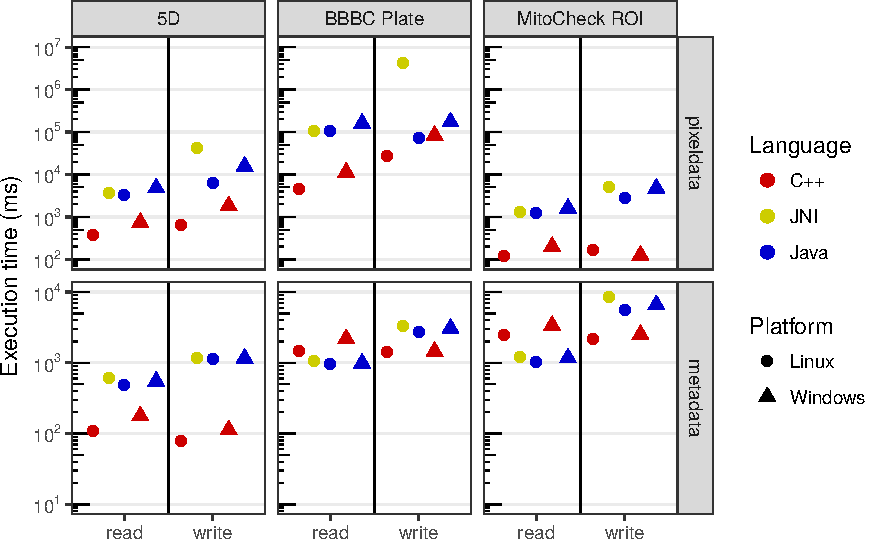
\includegraphics[width=\textwidth]{figures/files-suppfig5}
  \end{centering}
\end{frame}

\begin{frame}[fragile]
  \frametitle{Performance testing results (repeated)}
  \begin{centering}
    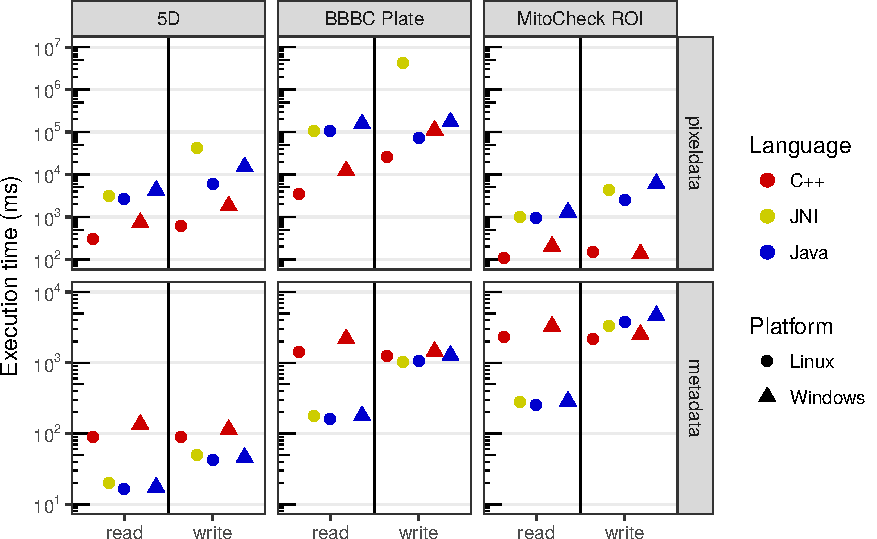
\includegraphics[width=\textwidth]{figures/files-suppfig6}
  \end{centering}
\end{frame}

\begin{frame}[fragile]
  \frametitle{Windows support}

  \begin{itemize}
  \item Added support for VS2015
  \item Dropped support for VS2012
  \item Added command line tools
  \item Numerous fixes and enhancements
  \end{itemize}
\end{frame}

\begin{frame}[fragile]
  \frametitle{Data model}

  Major features:
  \begin{itemize}
  \item Added 2015-01 and 2016-06 model support
    \pause
  \item Units
  \item Map annotations
  \item Model has feature and API parity in C++ and Java
  \item Native unit and quantity support
  \item C++ and Java model maintained together in a unified codebase
  \end{itemize}
  \pause

  \bigskip
  Minor features:
  \begin{itemize}
  \item BinData
  \item ROI transforms
  \end{itemize}
\end{frame}

\begin{frame}[fragile]
  \frametitle{TIFF readers and writers}

  \begin{itemize}
  \item added TIFF compression
  \item added default strip and tile size heuristic
  \item added IFD offset caching
  \item added OME-TIFF validity checks, metadata caching, file
    caching, plane element handling
  \end{itemize}

  \begin{lstlisting}[language=C++]
    writer.setCompression("lzw");
    writer.setInterleaved(false);
    writer.setTileSizeX(512U);
    writer.setTileSizeY(512U);
  \end{lstlisting}
\end{frame}

\begin{frame}[fragile]
  \frametitle{Additional changes}

  \begin{itemize}
  \item C++11/14
  \item Native unit and quantity support
  \item Updated examples
  \end{itemize}
  \pause

  \begin{lstlisting}[language=C++]
    typedef model::primitives::Quantity
      <model::enums::UnitsLength,
       model::primitives::PositiveFloat> PositiveLength;
    metadatastore.setPixelsPhysicalSizeX
      (PositiveLength(118.2, model::enums::UnitsLength::MICROMETER), 0);

    // C++11
    metadatastore.setPixelsPhysicalSizeX
      ({118.2, UnitsLength::MICROMETER}, 0);

    //  Low level Boost.Units
    micrometre_quantity len(118.2);
  \end{lstlisting}
\end{frame}

\begin{frame}[fragile]
  \frametitle{Python API}

  \begin{itemize}
  \item \url{https://github.com/ome/ome-files-py}
  \item Core: Python extension module that wraps the C++ API
  \item Can open image planes as NumPy arrays
  \item Work in progress: exposes a subset of \texttt{OMETIFFReader}
  \end{itemize}
  \begin{columns}
    \begin{column}{0.05\textwidth}
    \end{column}
    \begin{column}{0.65\textwidth}
      \centering
      \begin{lstlisting}[language=Python]
import ome_files
import matplotlib.pyplot as plt

reader = ome_files.OMETIFFReader()
reader.set_id("tubhiswt_C0.ome.tif")
pixels = reader.open_array(0)
reader.close()
plt.imshow(pixels, cmap="gray")
plt.show()
      \end{lstlisting}
    \end{column}
    \begin{column}{0.4\textwidth}
      \centering
      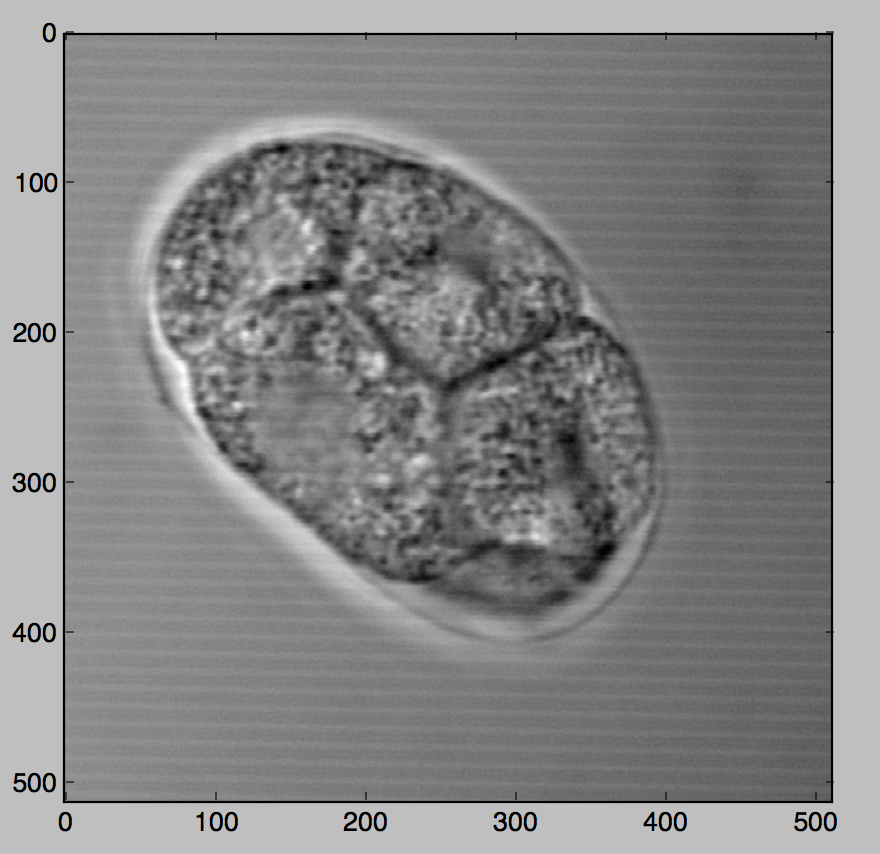
\includegraphics[width=0.85\textwidth]{figures/openbytes.png}
    \end{column}
  \end{columns}
\end{frame}

\begin{frame}[fragile]
  \frametitle{Python API: external metadata}

  \begin{columns}
    \begin{column}{0.6\textwidth}
      \centering
      \begin{lstlisting}[language=Python,basicstyle=\tiny\ttfamily]
import matplotlib.pyplot as plt
import pandas as pd
import datapackage
import ome_files
import ome_files.metadata as ofmd

reader = ome_files.OMETIFFReader()
reader.set_id("9I5TT808_F00000010.companion.ome")
pixels = reader.open_array(0)
plt.imshow(pixels, cmap="gray")
plt.show()
meta = ofmd.OMEXMLMetadata(reader.get_ome_xml())
reader.close()
cmso_annotations = [
  _ for _ in meta.get_map_annotations()
  if _.Namespace == "CMSO/dpkg"
]
ann = cmso_annotations[0]
paths = ann.Value.get("FilePath")
dp = datapackage.DataPackage(paths[0])
res_map = dict((_.descriptor["name"], _.local_data_path) for _ in dp.resources)
df = pd.read_csv(res_map["objects_table"])
df = df[df["time index"] == 0]
x, y = df["cell col"].values, df["cell row"].values
plt.scatter(x=x, y=y, s=100, edgecolors='b', facecolors='none')
plt.imshow(pixels, cmap="gray")
plt.show()
      \end{lstlisting}
    \end{column}
    \begin{column}{0.4\textwidth}
      \centering
      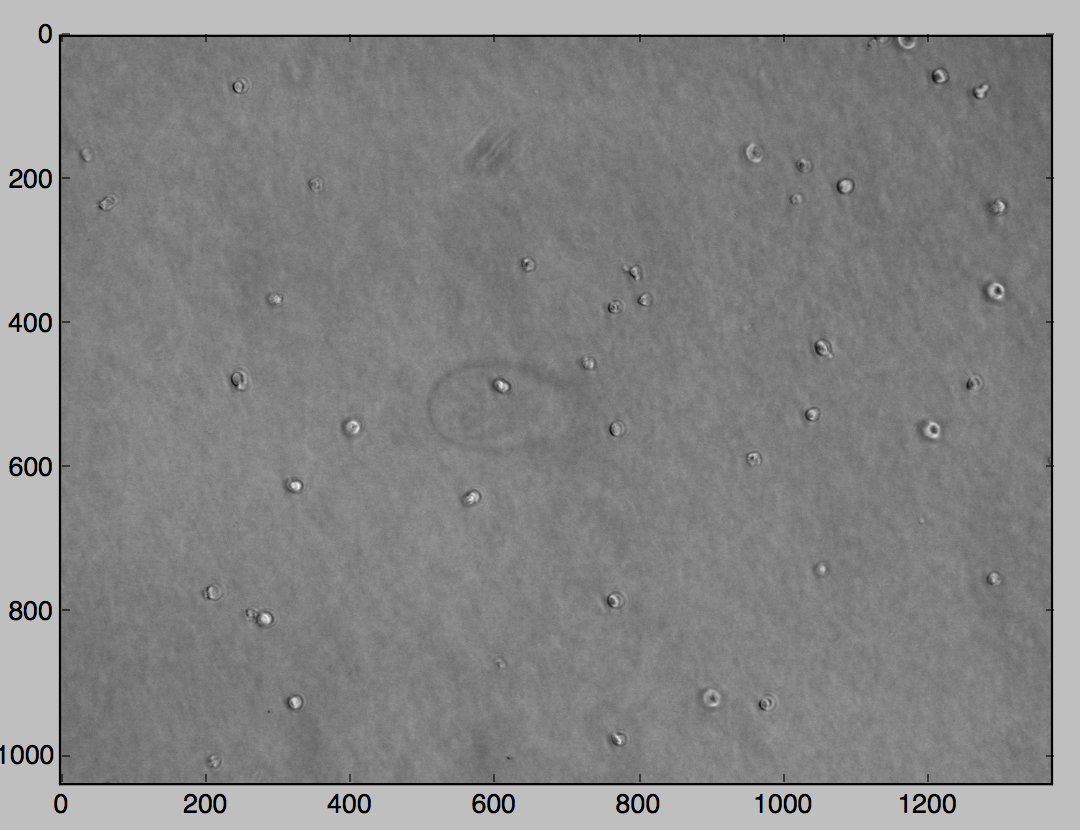
\includegraphics[width=\textwidth]{figures/tracking.png}\\
      \vspace{.5em}
      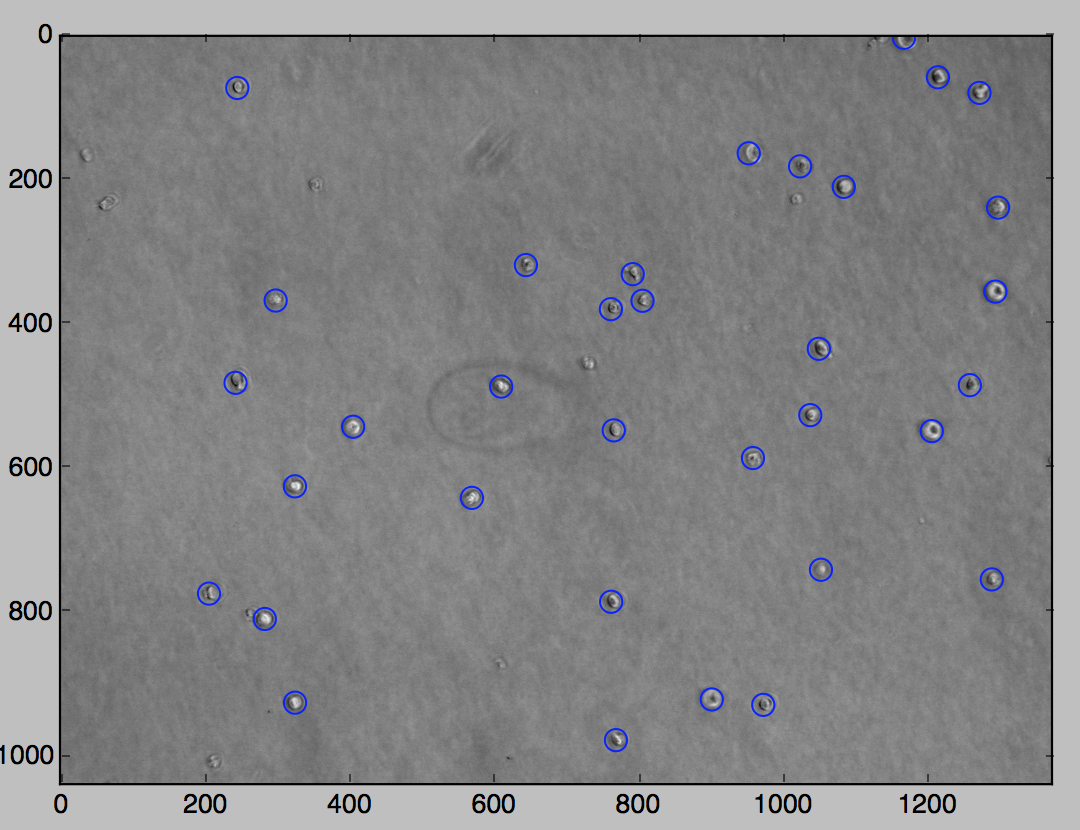
\includegraphics[width=\textwidth]{figures/overlay.png}
    \end{column}
  \end{columns}
\end{frame}

\begin{frame}[fragile]
  \frametitle{Future possibilities}

  \begin{itemize}
  \item Flexible model annotations
    \begin{itemize}
    \item \texttt{Modulo}
    \item Direct serialisation of custom annotations
    \end{itemize}
    \pause
  \item Options API (YAML?)
  \end{itemize}
\end{frame}

\begin{frame}[fragile]
  \frametitle{Feedback requested (and help required)}

  Feedback appreciated:
  \begin{itemize}
  \item Dropping support for VS2013 (deprecate then EOL?)
  \item Adding support for VS2017?
  \item Windows DLLs
  \end{itemize}
  \pause
  \bigskip
  Help or advice needed:
  \begin{itemize}
  \item Supporting Windows DLLs
  \end{itemize}
\end{frame}

\begin{frame}[fragile]
  \frametitle{Summary}

  OME Files C++ now supports:
  \begin{itemize}
  \item The latest OME-TIFF and OME Model versions
  \item Complete API parity with Bio-Formats (modulo \texttt{Modulo})
  \end{itemize}
  \bigskip
  Performance profiling shows:
  \begin{itemize}
  \item Pixel data performance exceeds Java performance
  \item Metadata writing exceeds Java performance
  \item Metadata reading mostly exceeds Java performance
  \end{itemize}
\end{frame}
\end{document}
